
\part{Voter model and reaction diffusion }
\noindent \begin{flushright}
\textit{I think that it is a relatively good approximation}\\
\textit{ to truth - which is much too complicated to }\\
\textit{allow anything but approximations \textemdash{} that}\\
\textit{ mathematical ideas originate in empirics.}\\
John von Neumann
\par\end{flushright}

In the previous sections, we have studied three equations describing
the \textit{macroscopic} evolution that was derived heuristically
with no \textit{microscopic} hypothesis. Indeed, obtaining a macroscopic
evolution equation from microscopic observations is one of the hardest
challenge of the modern science.

In 1955 Morrey \cite{Morrey1955} proposed the first serious mathematical
effort and bring to light the fundamental element to pass from microscopic
to macroscopic evolution equations: \textit{the suitable rescaling
of space and time}. 

In 1986 De Masi, Ferrari and Lebowitz \cite{DeMasi1987} studied interacting
spin systems on a lattice and proved that a perturbation occurs on
a fast time scale of order $\varepsilon^{-2}$ the macroscopic density
evolves according to an autonomous non-linear reaction-diffusion equation.

In the last decade Durrett et al \cite{cox_voter_2011,durrett_spatial_2014}
used De Masi - Ferrari - Lebowitz approach for the voter model to
study spatial evolutionary games. They considered games whose payoff
matrices are a perturbation of the voter model.

So in this part we first define the voter model, then perturb it and
at the end we simulate the related reaction diffusion equation in
$d=2$ for the prisoner dilemma. 

\section{The voter model\label{sec:The-voter-model}}

The voter model was introduced independently by Clifford and Sudbury
\cite{CLIFFORD1973} and by Holley and Liggett \cite{LiggettH1975}.
One can imagine that there is a \textquotedbl{}voter\textquotedbl{}
at each point on a lattice, that has an opinion with two possible
values, labelled $0$ and $1$. The opinions of any given voter changes
periodically (i.e., at independent exponential times) under the influence
of opinions of his neighbours. Specifically, for one of the chosen
voter's neighbours is chosen according to a given set of probabilities
and that individual's opinion is transferred to the chosen voter.

In more formal words the voter model is a Markov process $\eta_{t}$
with state space $S=\left\{ 0,1\right\} ^{\mathbb{Z}^{d}}$, where
$\mathbb{Z}^{d}$ is a d-dimensional integer lattice and the interactions
between an individual and its neighbours are given by an irreducible
symmetric probability kernel $p\left(x\right)$ that has covariance
matrix $\sigma^{2}I$. The evolution mechanism is described by saying
that $\eta\left(x\right)$ changes to $1-\eta\left(x\right)$ at rate:

\[
c\left(x,\eta\right)=\begin{cases}
\sum_{y}p\left(y-x\right)\eta\left(y\right) & \forall\eta(x)=0\\
\sum_{y}p\left(y-x\right)\left[1-\eta\left(y\right)\right] & \forall\eta(x)=1
\end{cases}
\]
where $p\left(x-y\right)\geq0$ for $x,y\in\mathbb{Z}^{d}$ and $\sum_{y}p\left(x-y\right)=1$
for $x\in\mathbb{Z}^{d}$ . In a more compact form:
\begin{equation}
c\left(x,\eta\right)=\sum_{y}p\left(y-x\right)\mathbf{1}_{\left\{ \eta\left(y\right)\neq\eta\left(x\right)\right\} }\label{eq:rate}
\end{equation}
where $\mathbf{1}$ is the indicator function of the set $\{\eta(y)\ne\eta(x)\}$.
It has some interesting properties:
\begin{itemize}
\item the configurations $\eta\equiv0$ and $\eta\equiv1$ are invariant
for the process, i.e. $c\left(x,\eta\right)=0$ $\forall x\in\mathbb{Z}^{d}$
if $\eta\left(x\right)=0\ \vee\ \eta\left(x\right)=1$. In terms of
the voter interpretation, there is no opinion flip when every voters
are in the same state. Moreover, for this reason the voter model is
never ergodic;
\item the evolution of the system does not change interchanging the roles
of 0's and 1's, i.e. $c\left(x,\eta\right)=c\left(x,\zeta\right)\quad\forall x\in\mathbb{Z}^{d}$
if $\eta\left(y\right)+\zeta\left(y\right)=1\quad\forall y\in\mathbb{Z}^{d}$.
\end{itemize}
Our question is what happens at infinite time and especially whether
or not 0's and 1's can coexist. Formally, calling $\eta_{t}\left(x\right)$
the state of the site $x$ at the time $t$, we say that \textit{coexistence}
occurs if: 
\[
\lim_{t\rightarrow\infty}\mathbb{P}[\eta_{t}(x)\neq\eta_{t}(y)]\neq0
\]
 while, if $\forall x,y\in\mathbb{Z}^{d}$ and all initial configurations,
we have: 
\[
\lim_{t\rightarrow\infty}\mathbb{P}[\eta_{t}(x)\neq\eta_{t}(y)]=0
\]
we say that \textit{clustering }(or \textit{consensus}) occurs. A
natural quantity of interest is the consensus time:

\[
T^{cons}\coloneqq\min\left\{ t:\ \eta_{t}\left(x\right)=k\quad\forall x\in\mathbb{Z}^{d}\quad with\ k=0,1\right\} 
\]

In this work we take a uniform probability kernel:
\[
p(y-x)=\begin{cases}
\frac{1}{2d} & if\ \left\Vert y-x\right\Vert _{1}=1\\
0 & otherwise
\end{cases},
\]
here $\left\Vert \cdotp\right\Vert _{1}$ is the Manhattan norm, i.e.
given $x,y\in\mathbb{Z}^{d}$ then $\left\Vert x-y\right\Vert _{1}=\sum_{i=1}^{d}\left|x_{i}-y_{i}\right|$.
Then, the transition rate is:
\[
c\left(x,\eta\right)=\frac{1}{2d}\sum_{y:\left\Vert y-x\right\Vert _{1}=1}\mathbf{1}_{\left\{ \eta\left(y\right)\neq\eta\left(x\right)\right\} },
\]
in other words the voter is influenced only by the nearest neighbours. 

\subsection{Coalescing random walks}

Furthermore, the voter model has a rich duality theory \cite{schertzer_brownian_2017,durrett_spatial_2014}.
The events can be represented by a rate 1 Poisson point process\footnote{A point process $\left\{ N\left(t\right),t\geq0\right\} $ is a stochastic
process \cite{daley2003an,wiki} that describes the occurrence over
time of random events in which the occurrences are revealed one-by-one
as time evolves. A Poisson process of rate $\lambda$ is a particular
point process satisfying the following four properties: 
\begin{itemize}
\item ${\textstyle N\left(0\right)=0}$;
\item has independent increments;
\item ${\displaystyle \mathbb{E}[N(t)]=\lambda t}+o\left(t\right)$, in
other words the probability that one event occurs in an interval of
length $t$ is proportional to $t$, while the probability that two
(or more) events occur in $t$ is negligible.
\end{itemize}
For the sake of clarity, the probability of the random variable $N\left(t\right)$
being equal to $n$ is given by the Poisson distribution$P\left[N(t)=n\right]=\frac{(\lambda t)^{n}}{n!}e^{-\lambda t}$.} of arrows along the edges of the lattice over time. Each arrow from
$x$ to $y$ at time $t$ indicates the voter at $x$ changing its
opinion at time $t$ to that of $y$. This is known as Harris\textquoteright{}
graphical construction. 

\begin{figure}

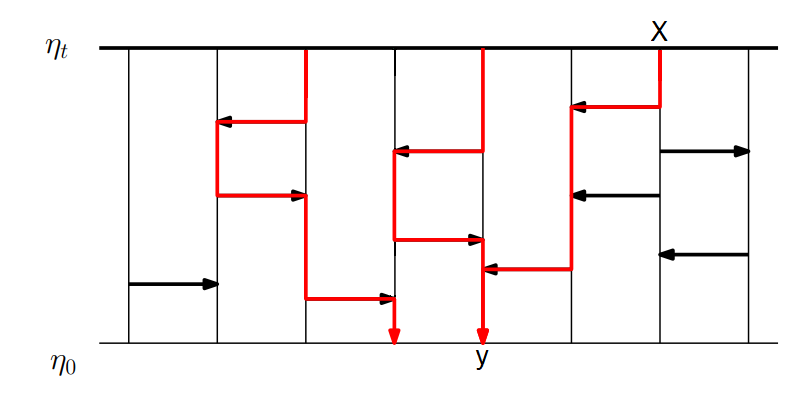
\includegraphics[width=0.7\textwidth]{immagini/harris}\caption{\label{fig:Harris}Example of Harris\textquoteright{} graphical construction
of the voter model on a one dimensional lattice (from \cite{schertzer_brownian_2017}) }

\end{figure}

To identify $\eta_{t}\left(x\right)$, we just need to work down the
graphical representation, i.e. trace the \textit{genealogy} of where
the opinion $\eta_{t}\left(x\right)$ comes from backward in time.
For example, in fig \ref{fig:Harris} to obtain the opinion at $t$
in $x$, we need to follow the arrows backward in time, until we reach
the origin $y$ of the walk at time $0$. It should be clear that
$\eta_{t}\left(x\right)=\eta_{0}\left(y\right)$. The genealogy line
$\pi_{t}^{x,t}$ for $\eta_{t}\left(x\right)$ is then a continuous
time random walk running backward in time that jumps at rate $1$.
In wider terms, we have:
\begin{equation}
\eta_{t}\left(x\right)=n_{t-s}\left(\pi_{s}^{x,t}\right).\label{eq:dual}
\end{equation}
Moreover, by construction we can observe that if two genealogy lines
collide at time $s$, i.e. $\pi_{s}^{x,t}=\pi_{s}^{x',t}$ for some
$s$, then the two random walks will stay together at \textit{earlier}
times. For these reasons we say that the voter model and the \textit{coalescing
random walks} are dual to one another. In other terms, we can say
that:
\begin{equation}
\mathbb{P}\left(\eta_{t}\left(x\right)=1\quad\forall x\in B\right)\text{=}\mathbb{P}\left(\eta_{0}\left(y\right)=1\quad\forall y\in\pi_{t}^{B}\right)\label{eq:dual_P}
\end{equation}
where $\pi_{t}^{B}$ is a set-valued dual process starting from each
point of $B$. 

Now we can formulate the Holley and Liggett's theorem \cite{LiggettH1975}:
\begin{thm}
\label{thm:voter}In $d\leq2$ the voter model approaches complete
consensus, i.e. as $t\to\infty$ $\mathbb{P}\left(\eta_{t}\left(x\right)=\eta_{t}\left(y\right)\right)=1$.
In $d\geq3$ if we assign opinions $1$ and $0$ independently to
sites with probabilities $u$ and $1-u$ then as $t\rightarrow+\infty$,
$\eta_{t}^{u}$ converges in distribution to $\eta_{+\infty}^{u}$,
a stationary distribution, $\nu_{u}$, in which a fraction $u$ of
the sites have opinion $1$. 
\end{thm}


\section{The voter model perturbations\label{sec:Voter-model-perturbation}}

Now, we want to analyse the connection between the interacting particle
system and the dynamical systems. Cox, Durrett and Perkins in \cite{cox_voter_2011}
rigorously showed this connection and formulated a reaction-diffusion
equation for the small perturbed voter model. 

In \cite{durrett_spatial_2014,cox_voter_2011} they studied a class
of interacting particle systems on $\mathbb{Z}^{d}$ whose transition
rate is a small perturbation of the transition rate of a voter model.
We choose the Birth-Death dynamics, so that the transition rate is:
\begin{equation}
c\left(x,\eta\right)=\sum_{y}p\left(y-x\right)\left[\mathbf{1}_{\left\{ \eta\left(y\right)\neq\eta\left(x\right)\right\} }+\varepsilon^{2}A_{\eta\left(x\right),\eta\left(y\right)}\right]\label{eq:perturbation}
\end{equation}

where the perturbation parameter is $0<\epsilon\ll1$ and, considering
the opinion $\eta\left(x\right)$ as the strategy of the voter in
$x$, $A_{\eta\left(x\right),\eta\left(y\right)}$ is the payoff of
the player in $x$ playing $\eta\left(x\right)$ against the player
in $y$ playing $\eta\left(y\right)$ in the game with the payoff
matrix \ref{eq:payoff}. In other words, we can see the transition
rate $c\left(x,\eta\right)$ as the payoff of the voter in $x$ playing
the strategy $\eta\left(x\right)$ against all the neighbouring voters
in $y$ playing $\eta\left(y\right)$. It can be shown that the perturbation
term is:
\begin{equation}
h_{i,j}\left(0,\eta\right)=\sum_{k}\sum_{x}\sum_{y}p\left(y-x\right)p\left(x\right)\mathbf{1}_{\left\{ \eta\left(x\right)=j,\eta\left(y\right)=k\right\} }A_{j,k}\label{eq:hij}
\end{equation}

In \cite{cox_voter_2011,durrett_spatial_2014} the following theorem
is enunciated and proved.
\begin{thm}
\label{thm:RDE-ips}Suppose $d\geq3$. Let $v_{i}\,:\,\mathbb{R}^{d}\rightarrow\left[0,1\right]$
be continuous with $\sum_{i\in\mathbb{Z}^{d}}v_{i}=1$. Let $\eta_{0}^{\varepsilon}$
be the initial conditions of the process with perturbed flip rates
with local density $v_{i}$ and let: 
\[
u_{i}^{\varepsilon}\left(x,t\right)=\mathbb{P}\left(\eta_{t\varepsilon^{-2}}^{\varepsilon}\left(x\right)=i\right)
\]
 If $x_{\varepsilon}\rightarrow x$ as $\varepsilon\to0$ then $u_{i}^{\varepsilon}\left(x_{\varepsilon},t\right)$
converges to $u_{i}\left(x,t\right)$, the solution of the following
system of partial differential equations: 
\begin{equation}
\frac{\partial u_{i}\left(x,t\right)}{\partial t}=\frac{\sigma^{2}}{2}\Delta u_{i}\left(x,t\right)+\phi_{i}\left(u\left(x,t\right)\right)\label{eq:rde}
\end{equation}
with initial condition $u_{i}\left(x,0\right)=v_{i}\left(x\right)$
and $\frac{\sigma^{2}}{2}$ depends on the topology of the lattice.
The reaction term: 
\begin{equation}
\phi_{i}\left(u\right)=\sum_{j\neq i}\left\langle \mathbf{1}_{\left\{ \eta\left(0\right)=j\right\} }h_{j,i}\left(0,\eta\right)-\mathbf{1}_{\left\{ \eta\left(0\right)=i\right\} }h_{i,j}\left(0,\eta\right)\right\rangle _{u}\label{eq:reactionterm}
\end{equation}
where $\left\langle \cdot\right\rangle $ is the expected value with
respect to the voter model stationary distribution $v_{u}$ in which
the densities are given by the vector $u$.
\end{thm}

Intuitively, the process is always close to the voter equilibrium
for the current density vector $u$, when on the time scale the voter
model runs at rate $\varepsilon^{-2}$ versus the perturbation at
rate $1$. Thus, the rate of change of $u_{i}$ depends on the nearby
sites assumed to be in that voter model equilibrium. We restrict to
dimensions $d\geq3$ because, as seen in theorem \ref{thm:voter},
the voter model does not have nontrivial stationary distributions
in $d\leq2$.

\section{The modified game}

Now, we can compute $\phi_{i}\left(u\right)$ for the Birth-Death
dynamics. Inserting the term \ref{eq:hij} in \ref{eq:reactionterm}
we obtain:
\begin{align*}
\phi_{i}\left(u\right) & =\left\langle \sum_{j\neq i}\mathbf{1}_{\left\{ \eta\left(0\right)=j\right\} }\sum_{k}\sum_{x}\sum_{y}p\left(y-x\right)p\left(x\right)\mathbf{1}_{\left\{ \eta\left(x\right)=i,\eta\left(y\right)=k\right\} }A_{i,k}\right.\\
 & -\left.\sum_{j\neq i}\mathbf{1}_{\left\{ \eta\left(0\right)=i\right\} }\sum_{k}\sum_{x}\sum_{y}p\left(y-x\right)p\left(x\right)\mathbf{1}_{\left\{ \eta\left(x\right)=j,\eta\left(y\right)=k\right\} }A_{j,k}\right\rangle \\
 & =\sum_{j\neq i}\sum_{k}q\left(j,i,k\right)A_{i,k}-q\left(i,j,k\right)A_{j,k}
\end{align*}
where the quantity: 
\[
q\left(i,j,k\right)=\mathbb{P}\left(\eta\left(0\right)=i,\eta\left(v_{1}\right)=j,\eta\left(v_{1}+v_{2}\right)=k\right)
\]
and $v_{1}$and $v_{2}$ are independent and chosen according to the
distribution $p$. We have for $i\neq j$:
\begin{align*}
q\left(i,j,k\right) & =p\left(0\mid v_{1}\mid v_{1}+v_{2}\right)u_{i}u_{j}u_{k}\\
 & +\mathbf{\mathbf{1}}_{\left\{ i=k\right\} }p\left(0,v_{1}+v_{2}\mid v_{1}\right)u_{i}u_{j}\\
 & +\mathbf{\mathbf{1}}_{\left\{ j=k\right\} }p\left(0\mid v_{1},v_{1}+v_{2}\right)u_{i}u_{j}
\end{align*}
 Here, we use Durret's notation where:
\begin{itemize}
\item $p\left(x\mid y\mid z\right)$ is the probability that the three random
walks never hit;
\item $p\left(x\mid y,z\right)$ is the probability that the walks starting
from $y$ and $z$ coalesce, but they do not hit the one starting
at $x$. 
\end{itemize}
So, inserting $q\left(i,j,k\right)$ in $\phi_{i}\left(u\right)$
, we have:
\begin{align*}
\phi_{i}\left(u\right) & =p\left(0\mid v_{1}\mid v_{1}+v_{2}\right)\sum_{j\neq i}\sum_{k}u_{i}u_{j}u_{k}\left(A_{i,k}-A_{j,k}\right)\\
 & +p\left(0,v_{1}+v_{2}\mid v_{1}\right)\sum_{j\neq i}u_{i}u_{j}\left(A_{i,j}-A_{j,i}\right)\\
 & +p\left(0\mid v_{1},v_{1}+v_{2}\right)\sum_{j\neq i}u_{i}u_{j}\left(A_{i,i}-A_{j,j}\right)
\end{align*}
It can be shown that:
\[
p\left(0,v_{1}+v_{2}\mid v_{1}\right)=p\left(0\mid v_{1},v_{1}+v_{2}\right)
\]
 and we have:
\begin{align*}
\phi_{i}\left(u\right) & =p\left(0\mid v_{1}\mid v_{1}+v_{2}\right)\sum_{j\neq i}\sum_{k}u_{i}u_{j}u_{k}\left(A_{i,k}-A_{j,k}\right)\\
 & +p\left(0\mid v_{1},v_{1}+v_{2}\right)\sum_{j\neq i}u_{i}u_{j}\left(A_{i,j}-A_{j,i}+A_{i,i}-A_{j,j}\right)
\end{align*}
The first term in the RHS is the replicator equation:
\[
\frac{du_{i}}{dt}=\sum_{j\neq i}\sum_{k}u_{i}u_{j}u_{k}\left(A_{i,k}-A_{j,k}\right)=\phi_{R}^{i}\left(u\right)
\]
If coalescing is impossible $p\left(0\mid v_{1}\mid v_{1}+v_{2}\right)=1$
and $p\left(0\mid v_{1},v_{1}+v_{2}\right)=0$, then $\phi_{i}=\phi_{R}^{i}$.
Now, let:
\[
M_{i,j}=\frac{p\left(0\mid v_{1},v_{1}+v_{2}\right)}{p\left(0\mid v_{1}\mid v_{1}+v_{2}\right)}\left(A_{i,j}-A_{j,i}+A_{i,i}-A_{j,j}\right)
\]
This matrix is skew symmetric $M_{i,j}=-M_{j,i}$ so $\sum_{i,j}u_{i}M_{i,j}u_{j}=0$
and we obtain:
\begin{align*}
\phi_{i}\left(u\right) & =p\left(0\mid v_{1}\mid v_{1}+v_{2}\right)\sum_{j\neq i}\sum_{k}u_{i}u_{j}u_{k}\left(A_{i,k}-A_{j,k}\right)\\
 & +p\left(0\mid v_{1}\mid v_{1}+v_{2}\right)\sum_{j\neq i}u_{i}u_{j}M_{i,j}
\end{align*}
We can easily prove that $\phi_{i}\left(u\right)$ is $p\left(0\mid v_{1}\mid v_{1}+v_{2}\right)$
times the RHS of the replicator equation for the modified game with
a payoff matrix $A+M$.

Moreover, it can be shown that:
\begin{align*}
p\left(0\mid v_{1}\right) & =2p\left(0\mid v_{1},v_{1}+v_{2}\right)+p\left(0\mid v_{1}\mid v_{1}+v_{2}\right)\\
p\left(0\mid v_{1}\right) & =\frac{1}{\kappa-1}
\end{align*}
where $\kappa$ is the number of neighbours of each site on the lattice.
Under the pair approximation, the coalescence of $0$ and $v_{1}$
is assumed independent of the coalescence of $v_{1}$ and $v_{1}+v_{2}$\cite{durrett_spatial_2014},
so: 
\[
\frac{p\left(0\mid v_{1},v_{1}+v_{2}\right)}{p\left(0\mid v_{1}\mid v_{1}+v_{2}\right)}=\frac{p\left(v_{1},v_{1}+v_{2}\right)}{p\left(v_{1}\mid v_{1}+v_{2}\right)}=\frac{1}{\kappa-2}
\]
Finally, the complete equation is:
\begin{align}
\frac{\partial u_{i}\left(x,t\right)}{\partial t} & =\frac{1}{\kappa}\Delta u_{i}\left(x,t\right)+p\left(0\mid v_{1}\mid v_{1}+v_{2}\right)\phi_{i}\left(u\right)\label{eq:RDE_durr}
\end{align}
where $\phi_{i}\left(u\right)$ is the replicator equation for the
modified game with a payoff matrix: 
\begin{equation}
A+M=\left\{ A_{i,j}+\frac{1}{\kappa-2}\left(A_{i,j}-A_{j,i}+A_{i,i}-A_{j,j}\right)\right\} \label{eq:A+M}
\end{equation}
 and by similar observation done in section \ref{sec:A-heuristic-derivation},
we assume $\frac{\sigma^{2}}{2}=\frac{1}{\kappa}$. Now the problem
is to evaluate the quantity $p\left(0\mid v_{1}\mid v_{1}+v_{2}\right)$.
The only way to do it is numerically, but this is beyond the scope
of this paper. The works of Durrett and Yuan Zhang suggest that $p\left(0\mid v_{1}\mid v_{1}+v_{2}\right)\in\left[0.32,\ 0.33\right]$.

Then, we can use this model for the prisoner's dilemma. Recalling
the payoff matrix: 
\[
A=\left(\begin{array}{cc}
1 & 0\\
b & 0
\end{array}\right)
\]
 the matrix $M$ has the following form:
\begin{align*}
M & =\left(\begin{array}{cc}
0 & \frac{1}{\kappa-2}\left(1-b\right)\\
-\frac{1}{\kappa-2}\left(1-b\right) & 0
\end{array}\right)
\end{align*}
 and so the modified payoff matrix is:
\[
A+M=\left(\begin{array}{cc}
1 & \frac{1}{\kappa-2}\left(1-b\right)\\
b-\frac{1}{\kappa-2}\left(1-b\right) & 0
\end{array}\right)
\]


\section{The simulations\label{sec:The-simulations-2}}

Now, we solve the equation \ref{eq:RDE_durr} for the prisoner's dilemma.
It is a parabolic partial differential equation, so we use the Crank-Nicolson,
seen in section \ref{sec:Parabolic-dynamic}. As done for the previous
models, we will study the dynamics \ref{eq:RDE_durr} on a two dimensional
plane $\left[0,L_{x}\right]\times\left[0,L_{y}\right]$ in a time
interval $\left[0,T\right]$. The equation is endowed with the initial
conditions:
\begin{align*}
u_{1}\left(x,y,0\right) & =u_{1}^{0}\left(x,y\right)\\
u_{2}\left(x,y,0\right) & =u_{2}^{0}\left(x,y\right)
\end{align*}
and we choose three forms of $u_{1}^{0}\left(x,y\right)$ and $u_{2}^{0}\left(x,y\right)$:
\begin{enumerate}
\item a random value between $0$ to $1$ for $u_{1}^{0}$ and $u_{2}^{0}=1-u_{1}^{0}$,
i.e.: 
\begin{align*}
\forall x,y\quad u_{1}^{0}\left(x,y\right) & =random\left[0,1\right]\\
\forall x,y\quad u_{2}^{0}\left(x,y\right) & =1-u_{1}^{0}\left(x,y\right)
\end{align*}
\item the population of the defectors is concentrated in a single point
in a sea of cooperators, i.e. for the cooperators:
\[
u_{1}^{0}\left(x,y\right)=\begin{cases}
1 & if\ x\neq\frac{L_{x}}{2}\ or\ y\neq\frac{L_{y}}{2}\\
0 & otherwise
\end{cases}
\]
 and for the defectors:
\[
u_{2}^{0}\left(x,y\right)=\begin{cases}
1 & if\ x=\frac{L_{x}}{2}\ and\ y=\frac{L_{y}}{2}\\
0 & otherwise
\end{cases};
\]
\item the portion of the defector agents is arranged as a delta distribution
surrounded by cooperators, i.e.:
\begin{align*}
u_{1}^{0}\left(x,y\right) & =\begin{cases}
1 & if\ x\neq\frac{L_{x}}{2}\\
0 & otherwise
\end{cases}\\
u_{2}^{0}\left(x,y\right) & =\begin{cases}
1 & if\ x=\frac{L_{x}}{2}\\
0 & otherwise
\end{cases}
\end{align*}
\end{enumerate}
And the chosen boundary conditions are zero, i.e. for $i=1,2$:
\[
u_{i}\left(0,0,t\right)=u_{i}\left(0,L_{y},t\right)=u_{i}\left(L_{x},0,t\right)=u_{i}\left(L_{x},L_{y},t\right)=0\quad\forall t\in\left[0,T\right].
\]


\subsection{Random initial condition}

First, we study the evolution of \ref{eq:RDE_durr} with a random
initial position of cooperators and defectors (fig \ref{fig:rand-2}). 

\begin{figure}
\subfloat[]{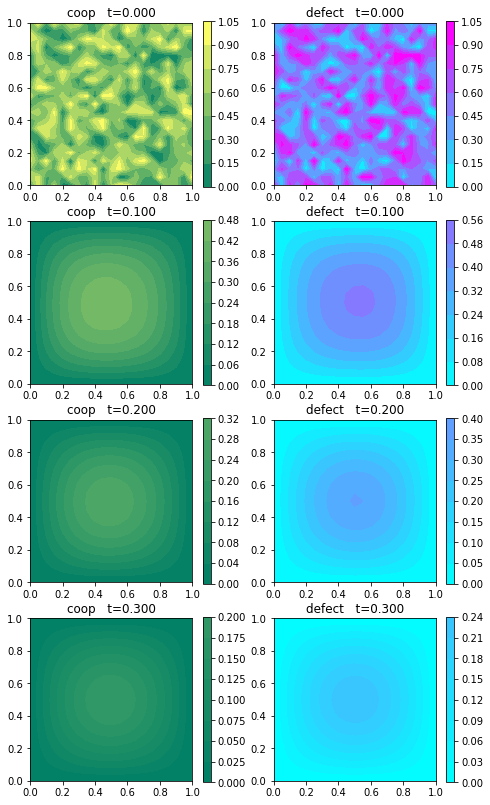
\includegraphics[width=0.5\textwidth]{immagini/durr-rand4}

}\subfloat[]{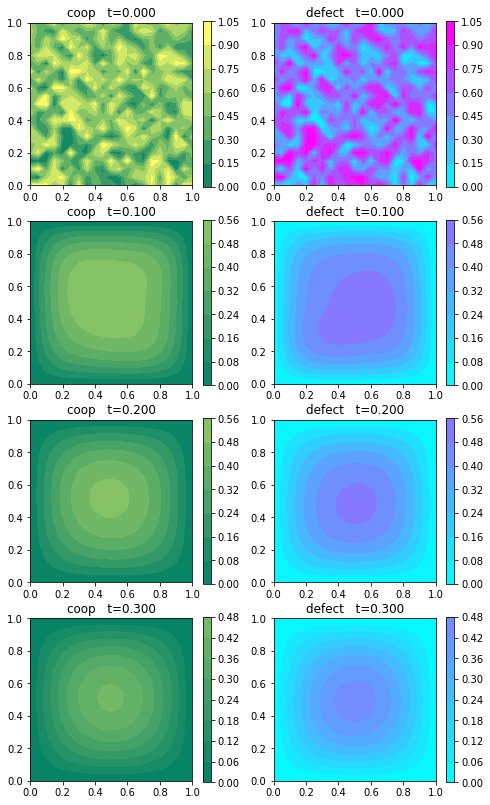
\includegraphics[width=0.5\textwidth]{immagini/durr-rand8}

}\caption{\label{fig:rand-2}Numerical solution of $u_{1}$ and $u_{2}$ in
$T=0.3$ and $L_{x}=L_{y}=20$ of \ref{eq:RDE_durr} using Crank-Nicolson
with $\kappa=4$ (A) and $\kappa=8$ (B). For both the methods we
set $N_{x}=N_{y}=20$, $dt=0.001$ and $b=1.85$.}
\end{figure}


\subsection{One defector in a sea of cooperators}

Secondly, we study the two equations setting at the starting time
the defectors in a single central point (fig \ref{fig:onedef-2}). 

\begin{figure}
\subfloat[]{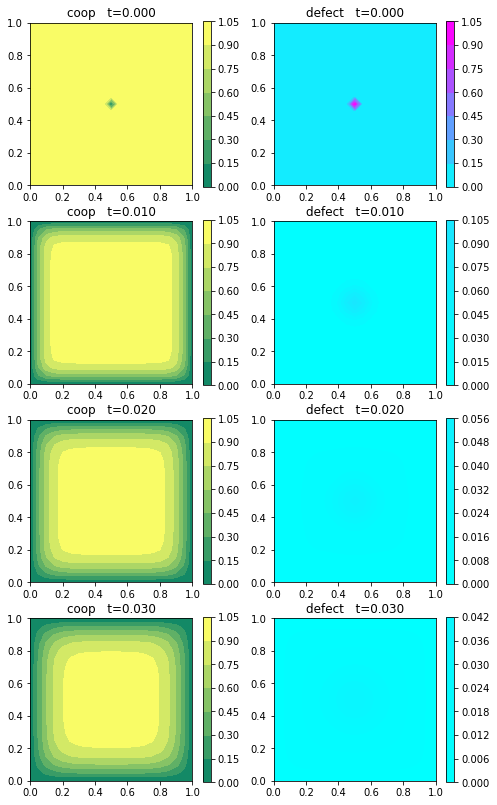
\includegraphics[width=0.5\textwidth]{immagini/durr-onedef4}

}\subfloat[]{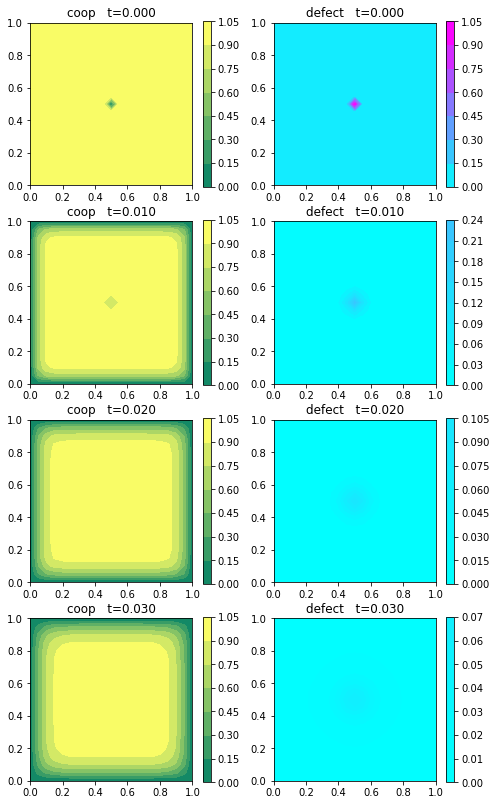
\includegraphics[width=0.5\textwidth]{immagini/durr-onedef8}

}

\caption{\label{fig:onedef-2}Numerical solution of $u_{1}$ and $u_{2}$ in
$T=0.3$ and $L_{x}=L_{y}=20$ of \ref{eq:RDE_durr} using Crank-Nicolson
with $\kappa=4$ (A) and $\kappa=8$ (B). For both the methods we
set $N_{x}=N_{y}=20$, $dt=0.001$ and $b=1.85$.}
\end{figure}


\subsection{Delta initial condition}

Finally, we analyse the two models, arranging the defectors in delta-type
function in the space surrounded by the cooperators, at the initial
time (fig \ref{fig:delta-2}). 

\begin{figure}
\subfloat[]{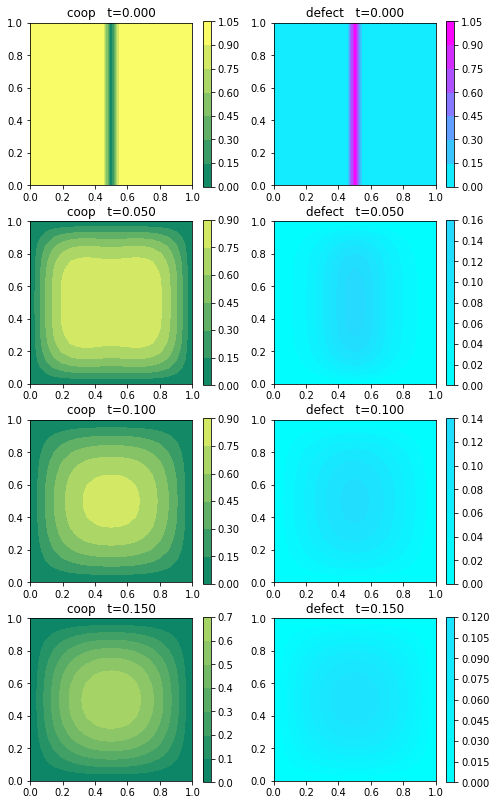
\includegraphics[width=0.5\textwidth]{immagini/durr-delta4}

}\subfloat[]{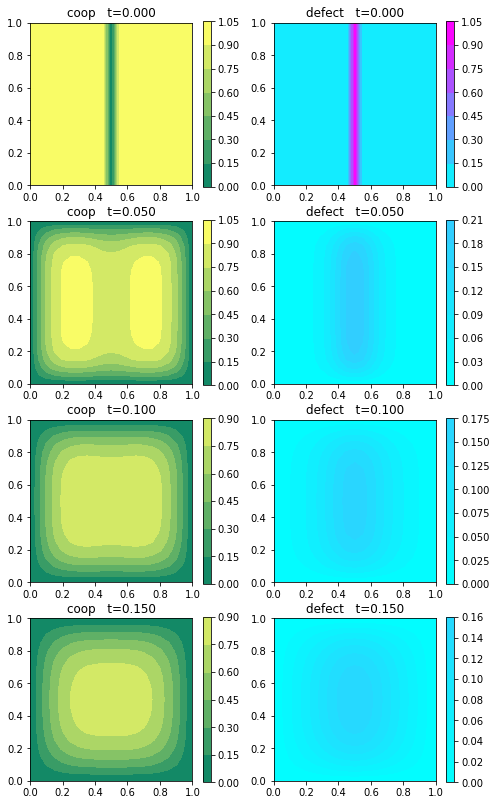
\includegraphics[width=0.5\textwidth]{immagini/durr-delta8}

}

\caption{\label{fig:delta-2}Numerical solution of $u_{1}$ and $u_{2}$ in
$T=0.3$ and $L_{x}=L_{y}=20$ of \ref{eq:RDE_durr} using Crank-Nicolson
with $\kappa=4$ (A) and $\kappa=8$ (B). For both the methods we
set $N_{x}=N_{y}=20$, $dt=0.001$ and $b=1.85$.}
\end{figure}


\subsection{Phase diagram and conclusions}

Here, it seems that the evolution is quite different from the previous
models, and in the last two cases the defectors do not invade the
whole of the space. But this is a fallacy, because we are considering
too short time frame predictions. Indeed, varying the value of $b$
and letting the evolution runs for $t\rightarrow+\infty$ (in practice
for $t$ sufficiently long) we can plot the phase diagrams of the
probability of a strategy.

\begin{figure}
\subfloat[]{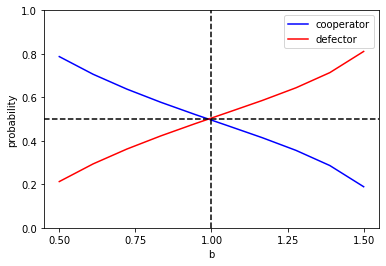
\includegraphics[width=0.5\textwidth]{immagini/durr4_phase}}\subfloat[]{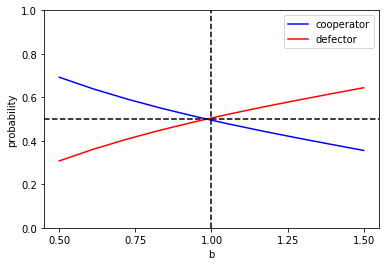
\includegraphics[width=0.5\textwidth]{immagini/durr8_phase}}\caption{Phase diagrams of the \ref{eq:RDE_durr} with 4 nearest neighbour
(A) and with 8 nearest neighbour (B).}
\end{figure}
Not so surprisingly, we observe a phase transition when $b=1$. Recalling
the payoff matrix:
\[
A=\left(\begin{array}{cc}
R & S\\
T & P
\end{array}\right)=\left(\begin{array}{cc}
1 & 0\\
b & 0
\end{array}\right)
\]
 we have a phase transition when the payoff of the defection (i.e.
the temptation $T$) becomes higher than the one for the cooperation
(i.e. the reward $R$). 
